\documentclass{article}

\usepackage{geometry}
\usepackage{graphicx}
\usepackage[ruled,vlined]{algorithm2e}

\usepackage{caption}
\usepackage{subcaption}

\geometry{margin=1in}

\author{Rohan Yadav}
\title{Final Project Writeup}
\date{}

\bibliographystyle{acm}

\begin{document}

\maketitle

\section{Background}

For my final project, I implemented a simple version of the common portrait mode feature supported by many mobile devices, and tuned the implementations for CPU and GPU targets.
%
In particular, I implemented components of portrait mode as described by Wadhwa et al~\cite{portrait} in the Halide domain specific language, and implemented schedules for both CPUs and GPUs.
%
My pipeline takes as input two stereo image pairs, and a foreground-background segmented image to define what portion of the image should remain in focus.
%
The goals of my project were to create aesthetically pleasing result images, and to tune the implementation to beat or equal the Halide autoschedulers.
%
Regarding quality of generated images, my pipeline generates good quality result images for a constrained set of inputs.
%
For performance, I compare my hand-tuned CPU schedule to the Mullapudi2016 and Adams2019 autoschedulers and find that my schedule has slightly better performance than both, and my hand-tuned GPU schedule equals the performance of the Li2018 GPU autoscheduler.

\section{Approach}

At a high level, an algorithm to perform a portrait mode style blur on an image must select what is the foreground and 
background of the image, and then blur the background component of the image. 
%
In order to get a more aesthetically pleasing in the background, it is beneficial to blur objects that are farther away
than those that are close to the camera.
%
To figure out what objects are far away, systems implement a form of depth estimation on the input images.
%
The reference system described by Wadhwa et al has the following high level stages.
%
\begin{enumerate}
    \item Apply an image segmentation network to identify the human in the foreground.
    \item Use dual-pixel hardware to collect a stereo image pair of the target photo.
    \item Use the stereo image pair to estimate the depth of each pixel in the image.
    \item Use the calculated depth information and segmented image to apply varying amounts of blur to the image.
\end{enumerate}

My implementation follows this high-level idea, but relaxes what components are produced by the pipeline or available from the underlying hardware.
%
In particular, I use an existing image segmentation network to perform foreground-background segementation, and treat this component as an input
to my pipeline.
%
Next, I do not have access to the raw dual-pixel (or Apple equivalent) data, so I used stereo image pairs from the Holopix50k~\cite{holopix} dataset.
%
These images have the same properties as the dual-pixel inputs to Wadhwa's pipeline -- they are vertically aligned and taken from a small distance apart.
%
After these modifications, my pipeline follows the same structure as Wadhwa's: I use the stereo image pairs to compute per-pixel depth information, 
and use the depth information along with the segmented image to produce the final output.
%
My full pipeline is described as psuedocode in Algorithm~\ref{alg:portrait}.
%
The tile minimization is performed via an align-and-merge algorithm, similar to the ideas used in Assignment 1.
%
Computation of disparity is performed by using similar triangle identities, as described by Wadhwa et al.
%
At a high level, at pixel, the closest tile that has a minimum difference from a tile around the pixel is found.
%
This minimum tile corresponds to that same pixel as viewed from the position of the camera taking the other
stereo image.
%
Therefore, the farther away the pixel and its match in the other image are, the closer the pixel is to the camera,
because things close to the camera translate the most when taking the photo from a different angle.
%
The different amount of blurs vary from 15-pixel wide blurs for very far objects, and 3-pixel wide blurs for close objects.
%
Synthetic noise is added back to the image so that the foreground and background have similar amounts of noise.
%
Otherwise, the blurred background appears to have less noise than the foreground.

My pipeline performs a simplified version of the steps performed by Wadhwa's pipeline.
%
In particular, they perform a confidence based version of the depth estimation procedure, and smooth the depth information with
a bilateral solver. Implementation of a bilateral solver was beyond my knowledge / Halide programming skills, so I used a bilateral
grid to perform edge-aware smoothing.

\begin{algorithm}
\caption{Portait Mode Pipeline}
\label{alg:portrait}
    \SetKwInOut{Input}{input}
    \SetKwInOut{Output}{output}

    \Input{Stereo image pair $I_l, I_r$, Segmented image $I_s$}
    \Output{Image with synthetic depth-of-field applied}
    \ForEach{\normalfont{pixel} $p \in I_l$}{
        $t \gets$ tile around $p$ \;
        $t' \gets$ tile in $I_r$ s.t. diff($t, t'$) is minimized \;
        minTile$(p) \gets $ coordinates of $t'$
    }
    disparity$(p)$ $\gets$ use coordinates at minTile$(p)$ to estimate disparity \;
    depth$(p) \gets$ inverse of disparity$(p)$ \;
    \tcc{Blur the depth information to smooth it out.}
    depth = medianBlur(depth) \;
    depth = bilateralGridBlur(depth) \;
    \tcc{Start to render the output image.}
    backBlurred = blur $I_l$ with different amounts, depending on depth \;
    noisy = apply synthetic noise to backBlurred \;
    portrait = select from noisy or $I_l$ depending on value in $I_s$ \;
    \Return{\normalfont{portrait}}
\end{algorithm}

\subsection{Results}

Figure~\ref{fig:ios} displays sets of inputs to my pipeline, the computed depth information, and the final output image.
%
Figure~\ref{fig:good} contains sets of additional output images from my pipeline that I thought were good quality result images.
%
As can been seen in the figures, the resulting images are indeed aesthetically pleasing, and look similar to outputs that may
be generated from a mobile phone's portrait mode setting.
%
The computed depth maps have mediocre resemblance to the depths that one might imagine from the input image, but were very noisy,
even after multiple forms of smoothing and blurring.
%
This noise arises from tile minimization approach to estimating the depth.
%
When all of the tiles around a target pixel are similar in the other stereo image due to repeated backgrounds, the matching
algorithm thinks that the pixel is in the same place in both images, i.e. it is very far from the camera.
%
This could be improved in the future by fully implementing the confidence based approach of Wadhwa et al -- such regions would be
marked as low confidence by the algorithm, and then lower confidence areas could be smoothed better.
%
However, the remaining noise in the depth map did not heavily affect the resulting blurred images.
%
This seems to indicate that the image segementation is more important than the quality of depth estimation for the quality
of the final output image.

One benefit of using a separate segmentation network was the variety of targets that could be segmented in comparison with Wadhwa's
pipeline.
%
The image segmentation network in Wadhwa's pipeline was trained for segmentation of humans.
%
If a human could not be identified in the photo, the pipeline fell back to using only dual-pixel depth map data to perform the
blurring.
%
In my situation, the segmentation network is treated as an input to the pipeline, and can thus be trained to segment any desired
inputs.
%
This allows me to generate portait mode style images for non-human targets, such as cats (shown below) and food (not shown).

The generated images in Figure~\ref{fig:good} are relatively high quality, and I believe that I achieved my goals in terms of output image quality.

\begin{figure*}
    \begin{subfigure}{\textwidth}
        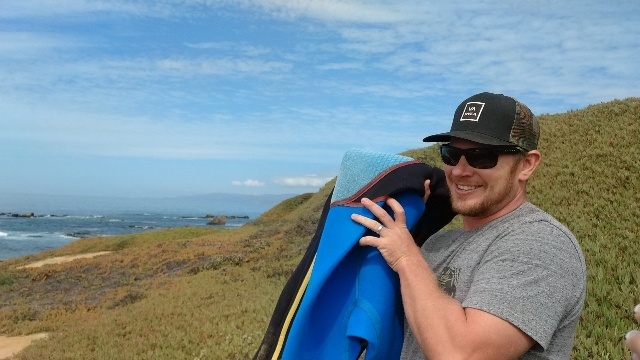
\includegraphics[width=0.5\textwidth]{../data/dude-left}
        
\includegraphics[width=0.5\textwidth]{../data/dude-seg-clean}
        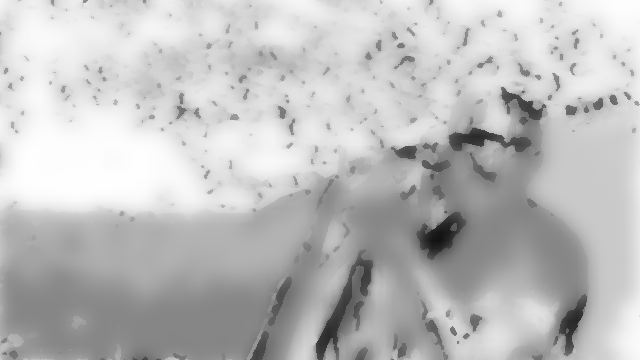
\includegraphics[width=0.5\textwidth]{../output/dude-depth}
        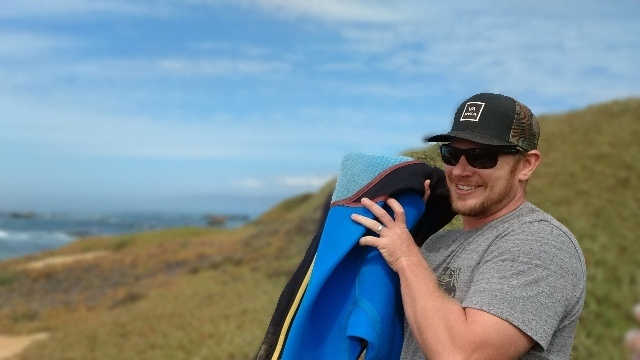
\includegraphics[width=0.5\textwidth]{../output/dude-portrait}
        \caption{Inputs and outputs for a picture of a guy.}
    \end{subfigure}

    \begin{subfigure}{\textwidth}
        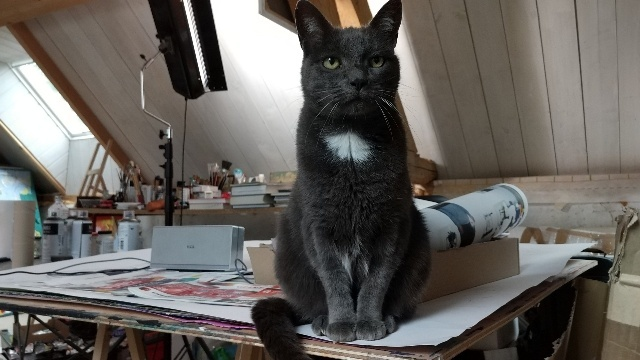
\includegraphics[width=0.5\textwidth]{../data/cat2-left}
        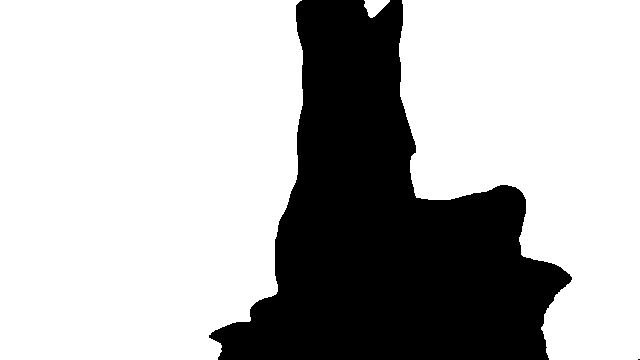
\includegraphics[width=0.5\textwidth]{../data/cat2-seg-clean}
        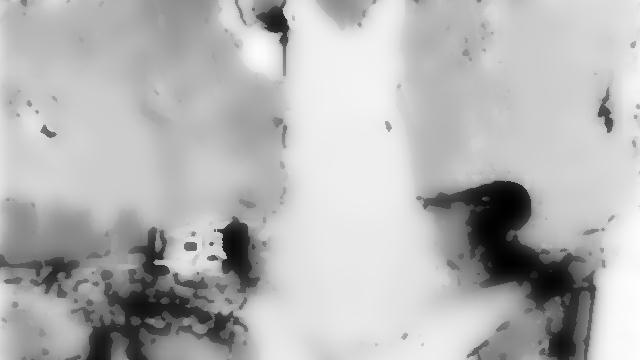
\includegraphics[width=0.5\textwidth]{../output/cat2-depth}
        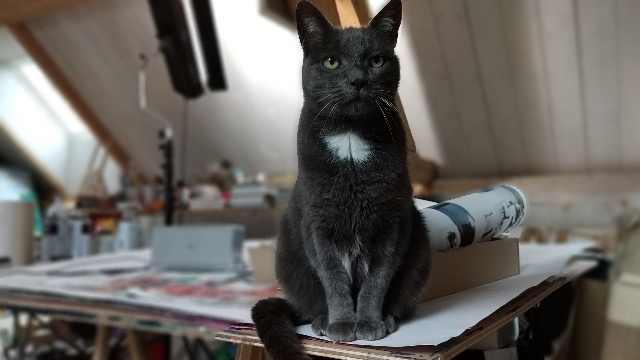
\includegraphics[width=0.5\textwidth]{../output/cat2-portrait}
        \caption{Inputs and outputs for a picture of a cat.}
    \end{subfigure}

    \caption{Two sets of example inputs and generated outputs from my pipeline. The top left image in each group of four is the left stereo image
    (the right stereo image looks mostly identical so it is excluded). The top right image is the input segmented image. The bottom left image is
    the depth map generated by my pipeline, where darker colors represent close objects. The final output is the bottom right image.}
    \label{fig:ios}
\end{figure*}

\begin{figure*}
        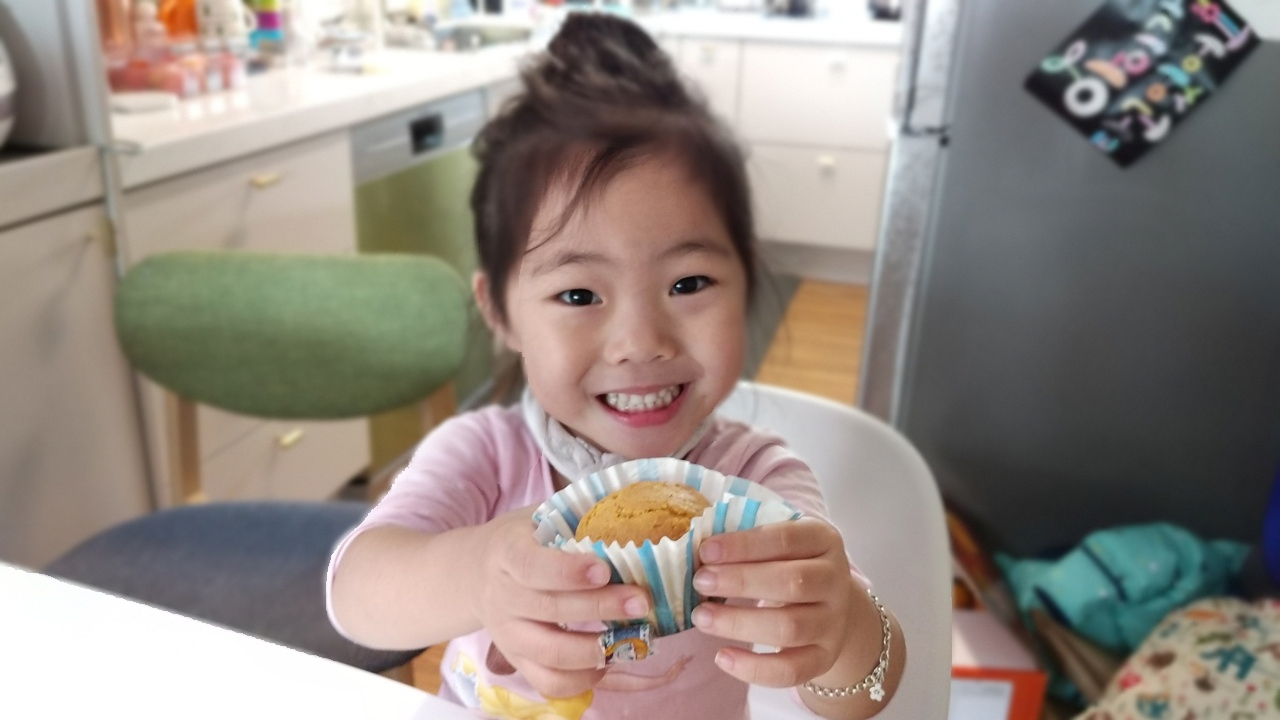
\includegraphics[width=0.5\textwidth]{../output/baby-portrait}
        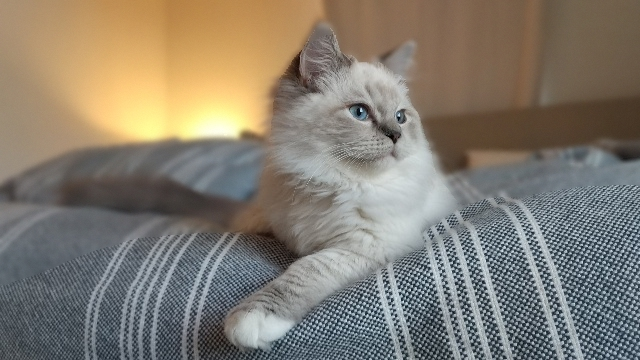
\includegraphics[width=0.5\textwidth]{../output/cat-portrait}
        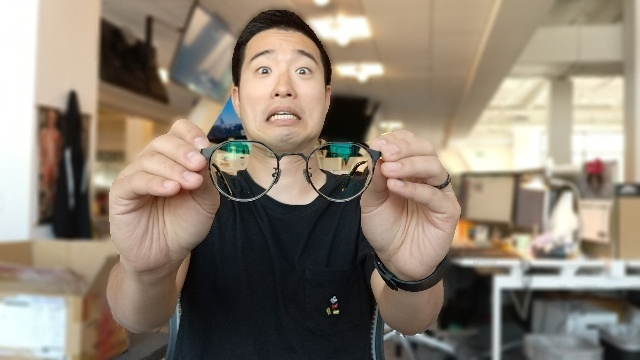
\includegraphics[width=0.5\textwidth]{../output/glasses-portrait}
        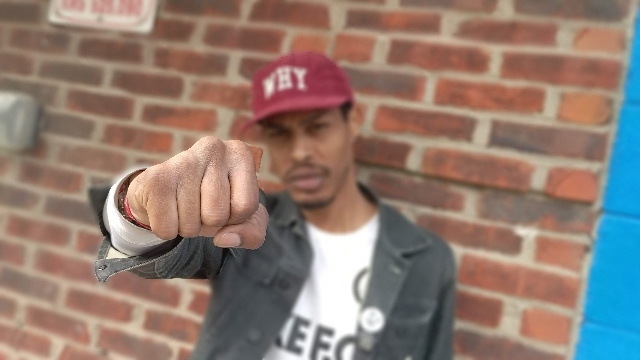
\includegraphics[width=0.5\textwidth]{../output/punch-portrait}
        \caption{Selected generated images of good visual quality.}
        \label{fig:good}
\end{figure*}

\section{Performance}

\subsection{Performance Optimization}

My performance optimization process was using Halide's scheduling primitives to optimize the performance of my pipeline.
%
My performance targets were the available Halide autoschedulers, as I was interested in seeing how well I could schedule the pipeline -- I did not
consider algorithmic changes to the pipeline to increase the performance.

\subsubsection{CPU Performance Tuning}

I recorded the execution time of my pipeline throughout the optimization process in Figure~\ref{fig:opti}.
%
At a moderate level of detail, the optimization steps I took were as follows:
\begin{enumerate}
  \item I started by computing all functions at the root, which took around 7.4s on a 512x512 image.
  \item I inlined all functions that did simple per-pixel operations, bringing me to 7s.
  \item I parallelized the different level blur operations, bringing me to 5.6s. Straightforward parallelization
      of chunks of rows led to this speedup.
  \item Parallelizing and reordering the computation of the aligning and merging process brough me to 4s. The computation was
      reordered to be more friendly to the memory layout of the images, and parallelism was done in a similar way as the blurs.
  \item I incorporated an existing schedule for the bilateral grid to get to 1.5s. This schedule was relatively straightforward,
      and paralellized a dimension of the grid and vectorized operations per grid point.
  \item I tuned this schedule more by tiling the phases, parallelizing over more components, and reordering the schedule for my data
      layout to get to 1.1s.
  \item I went back to vectorize the blur operations by giving each pixel a vector lnae, which led to a runtime of 0.63s.
  \item I parallelized and vectorized remaining stages of the pipeline (like the median blur) to get down to 0.5s.
  \item I was stuck here for a while, and noticed that the boundary conditions were not computed at the root. As I understood, this meant
      the boundary operations were all inlined, which potentially led to overhead when accessing them. I lifted these to the root and
      parallelized/vectorized them (rows/pixels) and saw a large speedup to 0.17s. At this point, the pipeline had equal performance to
      the Mullapudi2016 autoscheduler.
  \item The final optimization that had an affect was the use the \texttt{compute\_with} command to compute all of the different blur levels
      for a pixel at the same place to maximize the amount of data reuse. This dropped me down to 0.12s.
  \item I played around with the \texttt{rfactor} optimization to have reduction operations be parallelized, but this did not lead to
      any noticeable performance improvements.
\end{enumerate}

\begin{figure*}
    \centering
    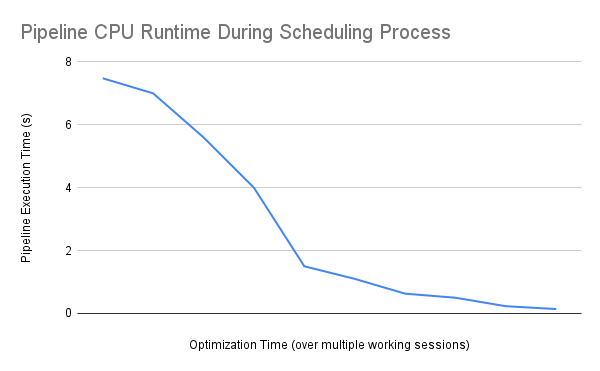
\includegraphics[width=0.75\textwidth]{cpu_opti_graph}
    \caption{Optimization progress of the pipeline on CPU on my MacBook.}
    \label{fig:opti}
\end{figure*}

\subsubsection{GPU Performance Tuning}

The performance tuning process for GPUs was definitely less interesting than the CPU optimization process.
%
The initial (dumb) strategy of performing all computations at the root and parallelizing all operations so that
each pixel was mapped to a GPU thread was enough to equal the performance of the Li2018 autoscheduler.
%
I made several attempts to apply optimizations that performed well for CPUs for the GPU schedule that resulted
in no improvements.
%
Most surpisingly, using \texttt{rfactor} to parallelize reduction operations had no benefit, even though without
that scheduling operation, reductions over the entire image were occurring on a single (slow) GPU thread.

\subsection{Experiments}

\subsubsection{Experimental Setup}

I performed experiments on two different machines. The first is my local MacBook, containing a 4-core Intel CPU. 
%
The second is a node in the Sapling development cluster at Stanford, with an NVIDIA Tesla P100 GPU.

\subsubsection{Results and Analysis}

Overall results are displayed in Figure~\ref{fig:results}.
%
Figure~\ref{fig:speedup} includes a speedup plot of my pipeline with increasing numbers of CPU cores.
%
Figure~\ref{fig:table} is a shootout experiment of my schedule for CPUs and a GPU against the autoschedulers distributed as part of Halide.

Figure~\ref{fig:speedup} shows that the pipeline achieves perfect speedup until 4 cores, and then flattens out at 8 cores.
%
This is expected, as my laptop only has 4 cores. At 8 "cores", hyperthreads are being used.
%
This application is compute bound, as the large blur operations (up to 15 wide) and "align and merge" style operations perform many operations
for each data element loaded from memory.
%
Since the application is compute bound, it achieves perfect speedup as more compute resources are given to it, as can be seein in Figure~\ref{fig:speedup}.
%
Once moving to hyperthreads, additional benefits are not as pronounced as the hyperthreads can only hide memory latency, not provide extra compute.

The results in Figure~\ref{fig:table} show that my schedule for CPU's and a GPU is slightly faster than all of the autoschedulers, which
improves on my initial goal of equaling the autoschedulers' performance.
%
In general, it was difficult to interpret the schedules chosen by the autoschedulers in order to contrast the differences in scheduling,
from either the generated schedule or emitted for-loop structure.
%
At a high level, the autoschedulers attempted more exotic methods of inlining and computing functions at other functions.
%
In the end, these were slightly slower than a somewhat more straightforward schedule that computed many functions at the root.

\begin{figure*}
    \begin{subfigure}{0.5\textwidth}
        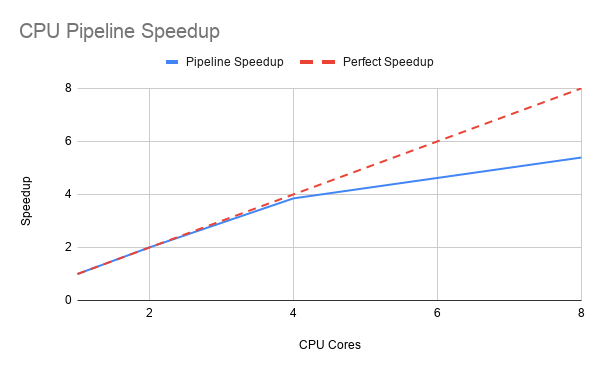
\includegraphics[width=\textwidth]{cpu_speedup}
        \caption{Speedup of pipeline with more CPU cores}
        \label{fig:speedup}
    \end{subfigure}
    \begin{subfigure}{0.5\textwidth}
        \centering
        \begin{tabular}{|c|c|c|}
            \hline
            Scheduler & CPU Time (s) & GPU Time (s) \\ 
            \hline
            Rohan & 0.12 & 0.019 \\
            \hline
            Mullapudi2016 & 0.15 & X \\
            \hline
            Adams2019 & 0.23 & X \\
            \hline
            Li2018 & 0.14 & 0.021 \\
            \hline
        \end{tabular}
        \caption{Performance of each scheduler on CPUs (my MacBook) and a GPU (Sapling) in seconds. 'X' indicates the scheduler did not support the corresponding target.}
        \label{fig:table}
    \end{subfigure}
    \caption{Overall performance results.}
    \label{fig:results}
\end{figure*}

\bibliography{biblio.bib}

\end{document}
